\documentclass{article}
\usepackage[magyar]{babel}
\usepackage{t1enc}
\usepackage[inline]{enumitem}
\usepackage{float}
\usepackage{subcaption}
\usepackage{array}
\usepackage{colortbl}
\usepackage{wrapfig}
\usepackage{multirow}
\usepackage{lipsum}
\usepackage{graphicx}
\usepackage[dvipsnames]{xcolor}

\setlistdepth{5}


\setlist[enumerate,1]{label=(\arabic*)}
\setlist[enumerate,2]{label=(\alph*)}
\setlist[enumerate,3]{label=(\roman*)}
\setlist[enumerate,4]{label=(\alph*)}
\setlist[enumerate,5]{label=(\roman*)}

\renewlist{enumerate}{enumerate}{5}

\begin{document}
\listoffigures

---------------------------------------------------------------------------------------------------\\\\
References:\\
\ref{figure}\\
\subref{subfig1}\\
\subref{subfig2}
\\\\
First list:\\
\hspace{1cm}
\begin{itemize*}[itemjoin*={ és \\}]
\item[+]ex.item1\\
\item[+]ex.item2\\
\item[+]ex.item3
\end{itemize*}\\

Second list:
%1st
\begin{enumerate} 
\item ex.itema
\begin{enumerate}
\item ex.itemb
\begin{enumerate}
\item ex.itemc
\begin{enumerate}%[label=\alph*.]
\item ex.itemd
\begin{enumerate}
\item ex.itemfifthlvl
\item ex.itemfifthlvls
\end{enumerate}
\item ex.iteme
\end{enumerate}
\item ex.itemf
\end{enumerate}
%2nd
\item ex.itemg
\end{enumerate}
\item ex.itemh
\begin{enumerate}
\item ex.itemi
\item ex.itemj
\end{enumerate}
\end{enumerate}
\newpage
\lipsum[1]\\ \\
\ref{counted}\\
\ref{uncounted}
\begin{enumerate}[resume]
%
\item ex.continues
\begin{enumerate}
\item ex.itemk
\begin{enumerate}
\item ex.iteml
\begin{enumerate}
\item[+] ex.itemm \stepcounter{enumiv}
\label{uncounted}
\item ex.itemn
\label{counted}
\item ex.itemo
\end{enumerate}
\item ex.itemp
\end{enumerate}
\item ex.itemq
%
\end{enumerate}
\item ex.continues2
\begin{enumerate}
\item ex.itemr
\item ex.items
\end{enumerate}
\end{enumerate}
%
-\\
Third list:
\begin{description}[style=nextline]
\item[]
\lipsum[1]
\item[slanted]
\lipsum[1]
\item[this should be very long, more than a line, so I will write here some text, this doesn't make any sense]\lipsum[1]
\end{description}
\newpage


\begin{figure}
\caption{Figure}
\label{figure}
\begin{wrapfigure}{l}{0.35\textwidth}

\begin{subfigure}{4cm}
\subcaption{Cormorant}
\label{subfig1}
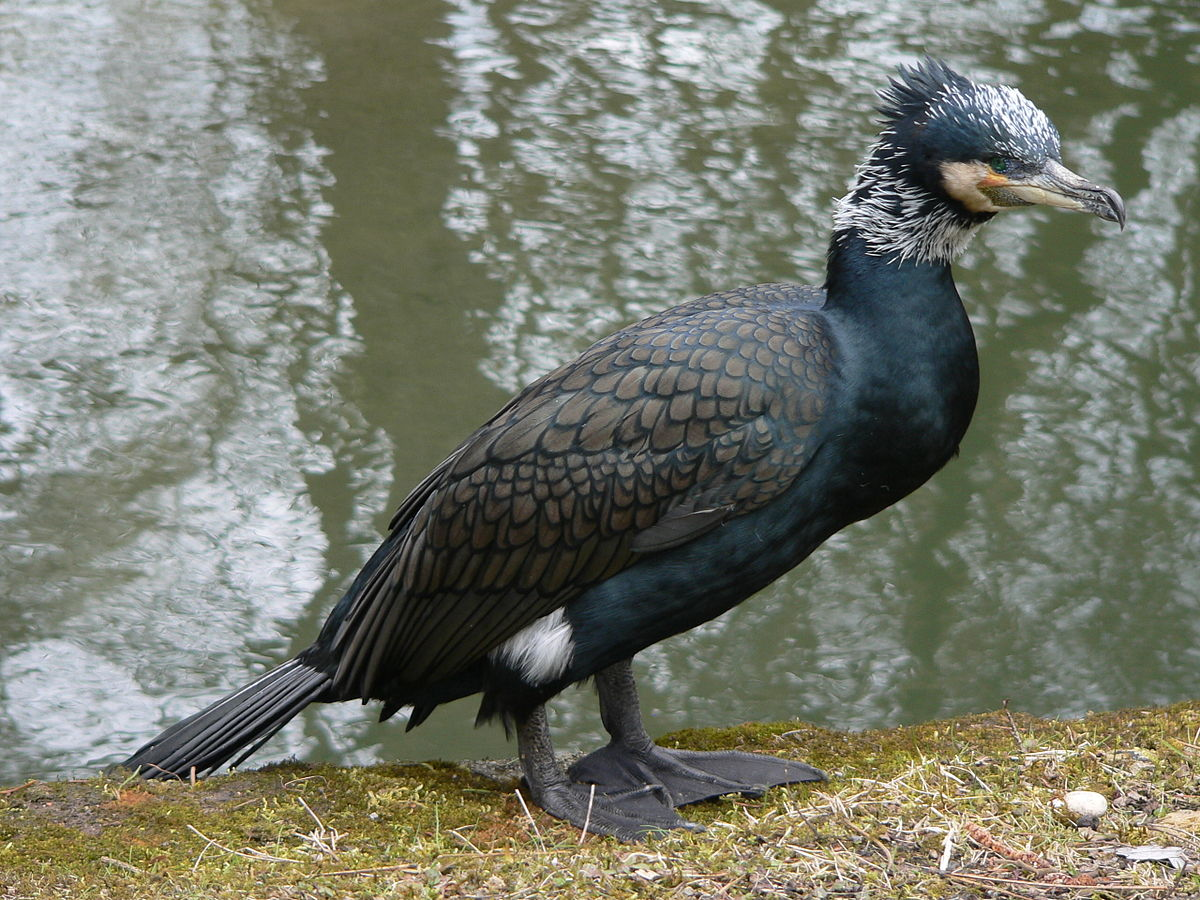
\includegraphics[scale=0.1]{forraskepek/kep1.jpg}
\end{subfigure}

\lipsum[6]

\begin{subfigure}{4cm}
\subcaption{Cormorant upside down}
\label{subfig2}
\scalebox{1}[-1]{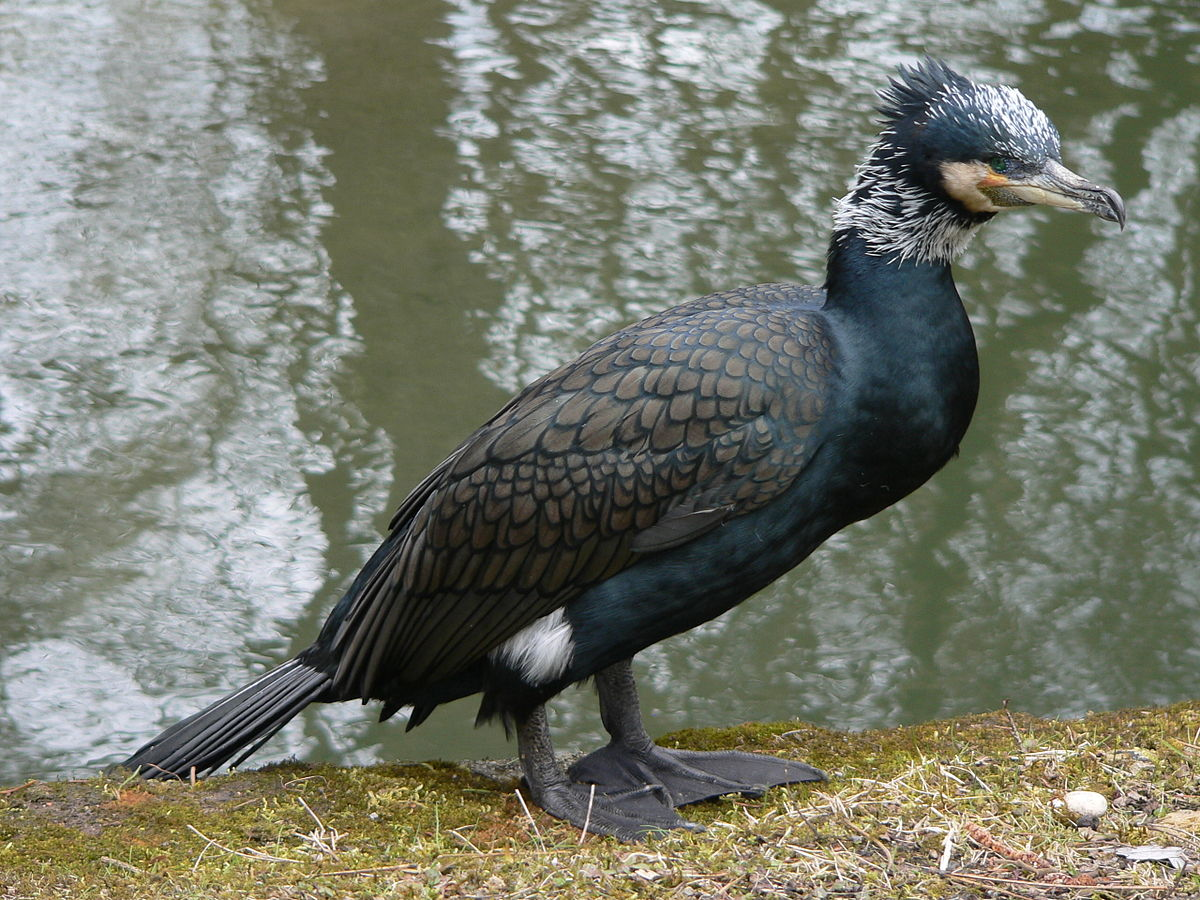
\includegraphics[scale=0.1]{forraskepek/kep1.jpg}}
\end{subfigure}
\end{wrapfigure}
\lipsum[1-3]
\end{figure}

\clearpage

\begin{tabular}{p{3em}||lll|}
 & egy  & kettő & három \\ \hline\hline
Helló világ! & négy & öt & hat \\ \cline{2-4}
 & hét & nyolc & kilenc \\ \cline{2-2}\cline{4-4}
lórum ipse & tíz & & tizenkettő\\ \hline
\end{tabular}
\\\\\\\\
\begin{tabular}{l|l|l}
egy  & kettő & három \\ \hline 
\rowcolor{Apricot}négy & öt & hat \\ 
\rowcolor{Orchid}hét & nyolc & kilenc \\
\rowcolor{Apricot}tíz & tizenegy & tizenkettő\\ 
\end{tabular}
\\\\\\\\

\begin{wraptable}{l}{3cm}
\begin{tabular}{l!{\color{red}\vrule}l|l|}

egy & \multicolumn{2}{c|}{kettő} \\ \hline
\multirow{2}{2em}{négy} & öt & hat \\ \cline{2-3}
 &\multicolumn{2}{c|}{\multirow{2}{2em}{nyolc}} \\ \cline{1-1}
tíz& \multicolumn{2}{c|}{}\\ \hline
\end{tabular}
\end{wraptable}
\lipsum[2]
\end{document}

